\section{Generale / Membro}
Questa sezione contiene tutte le informazioni di carattere generale dell'applicazione: è quindi indicata a tutti gli utenti che devono svolgere svolgere compiti base nell'applicazione. Ad esempio modificare le proprie impostazioni o tenere sotto controllo le rilevazioni visualizzate sotto forma di grafico o di correlazione all'interno della \glock{webapp}.

\subsection{Autenticazione}
Per visualizzare il tutorial recati al seguente link: 
\url{}

\subsection{Autenticazione a due fattori}
Per visualizzare il tutorial recati al seguente link: 
\url{}

\subsection{Visualizzazione dashboard e supporto tecnico}
Per visualizzare il tutorial recati al seguente link: 
\url{}

\subsection{Modifica impostazioni}
\url{}

\subsection{Configurazione Telegram}
	Per usufruire delle funzionalità di alert è necessario scaricare l'applicazione Telegram dallo store sul proprio dispositivo.
	Dopo aver avviato l'applicazione è necessario entrare nelle impostazioni cliccando prima sul menù ad hamburger in altro a sinistra sullo schermo.
	\begin{figure}[H]
		\centering
		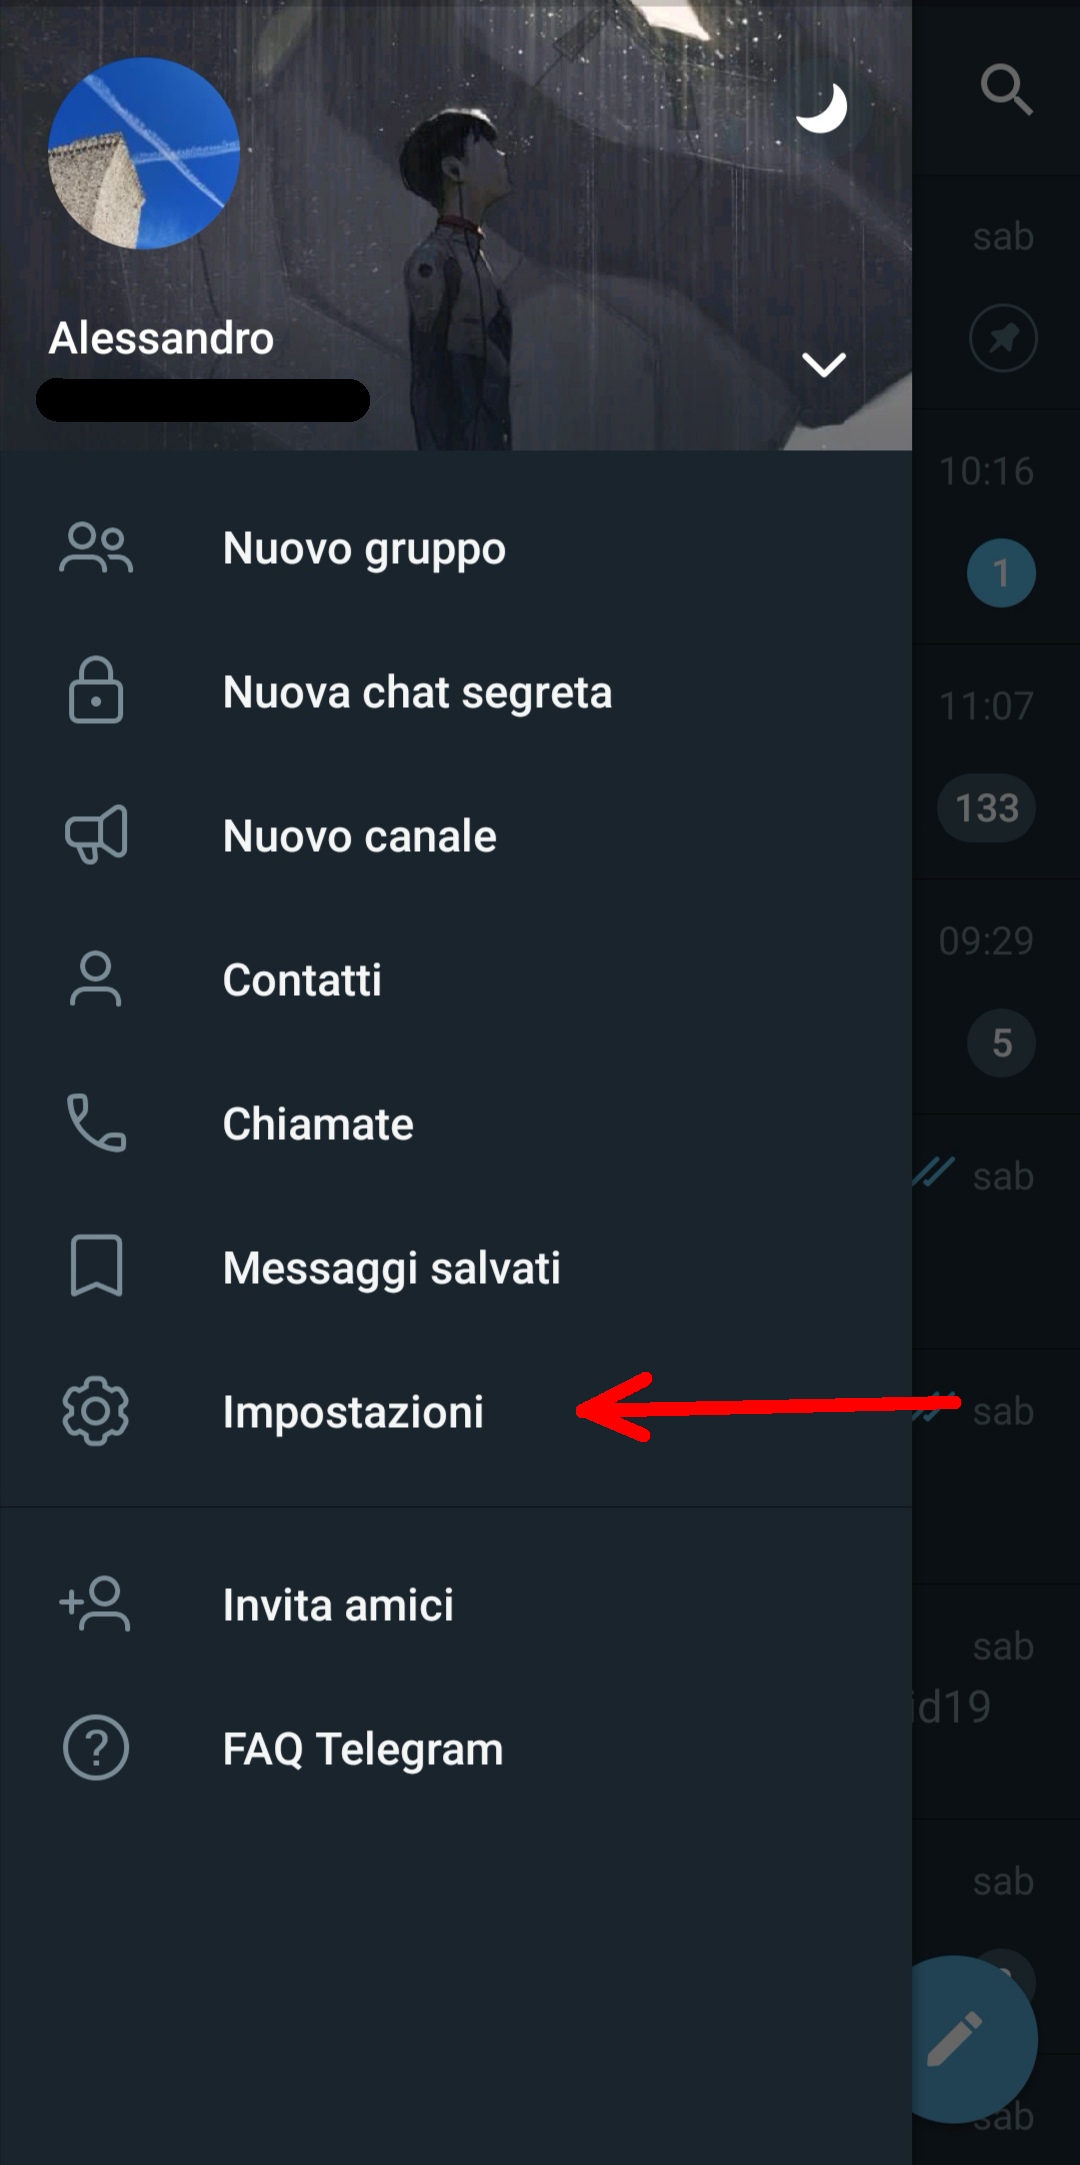
\includegraphics[scale=0.100]{res/images/telegram1.jpg}
		\caption{Come entrare nella sezione impostazioni}
		\label{Screenshot1}
	\end{figure}
	\newpage
	In seguito è necessario cliccare nel punto indicato dalla freccia per poter inserire e/o modificare il proprio username
	\begin{figure}[H]
		\centering
		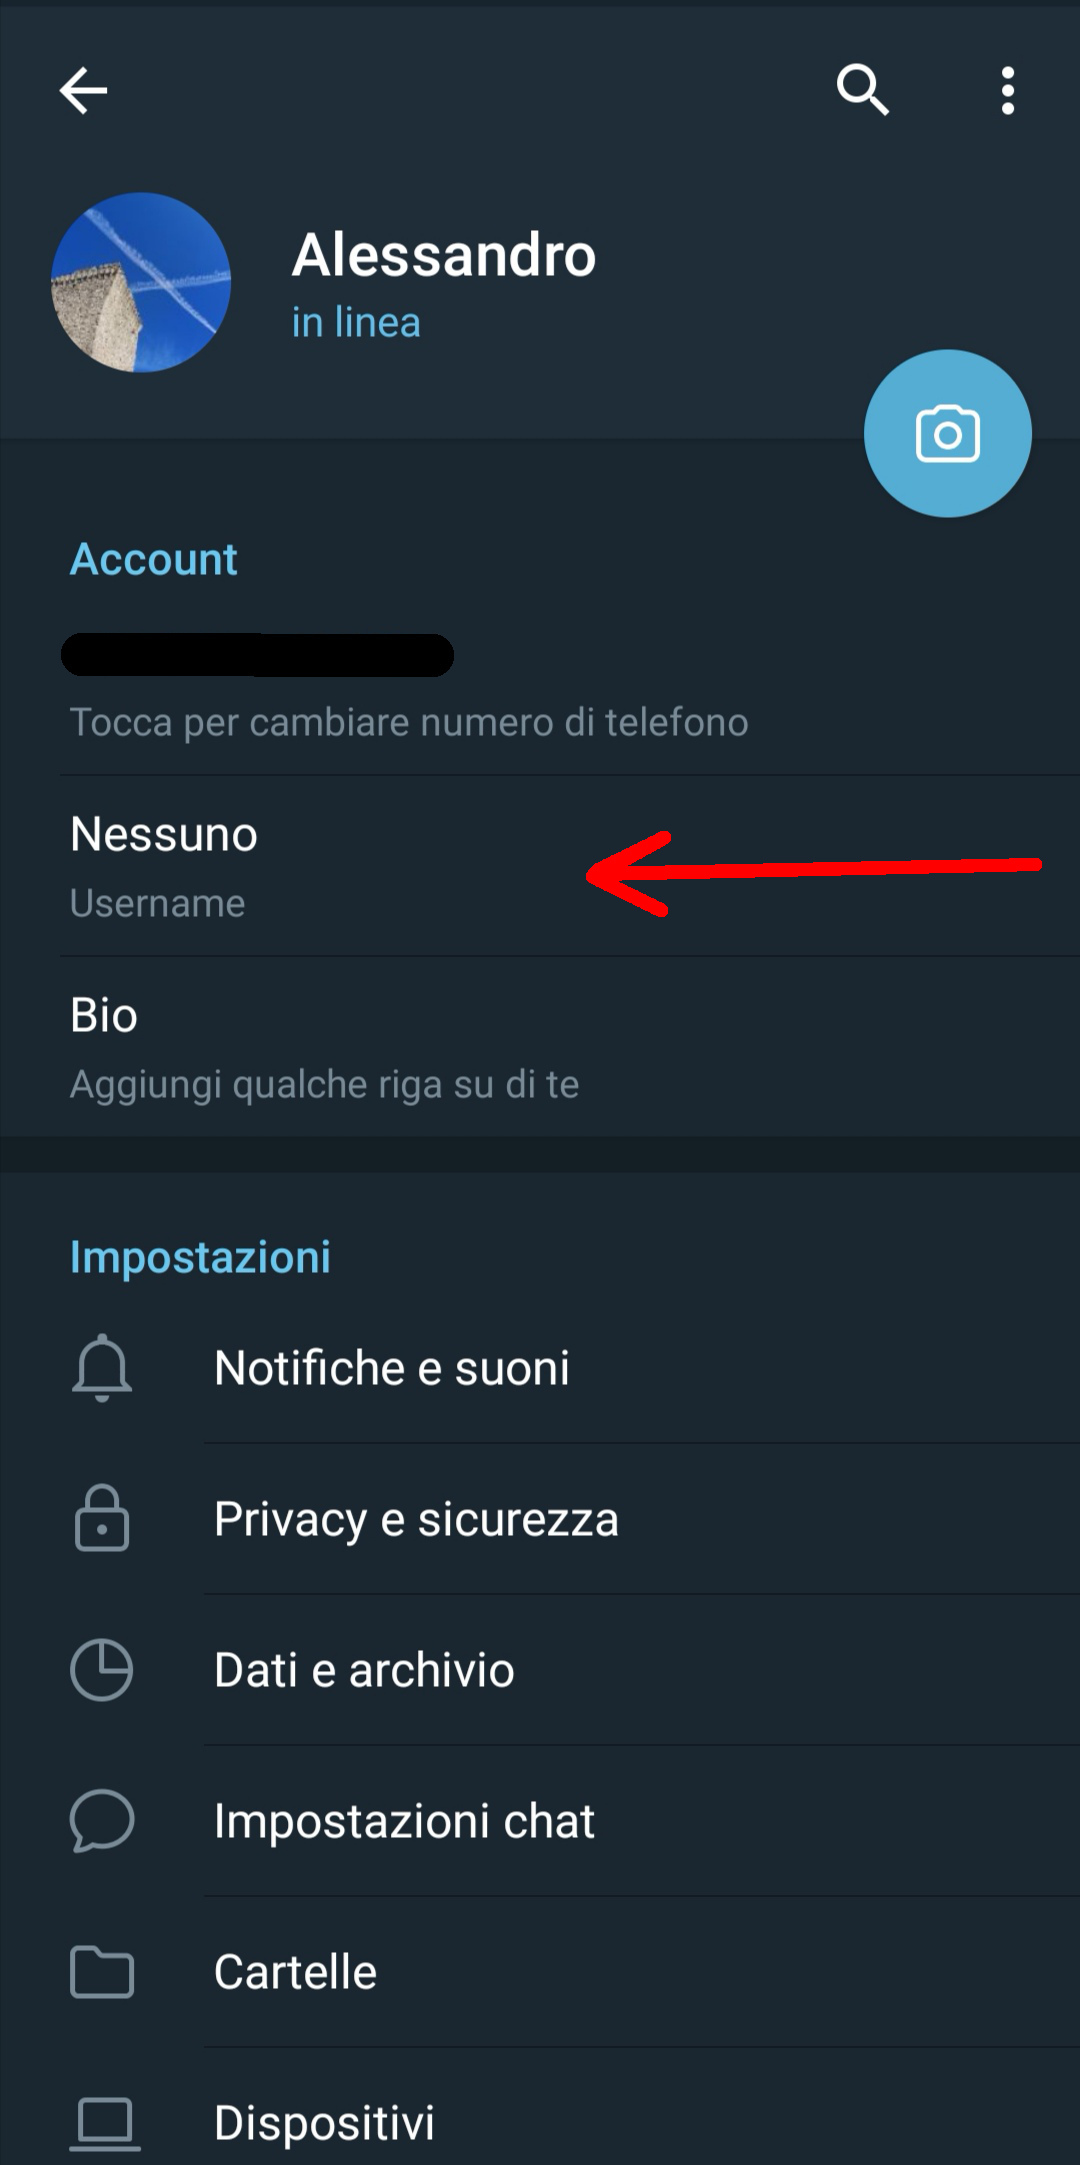
\includegraphics[scale=0.100]{res/images/telegram2.jpg}
		\caption{Come inserire uno username}
		\label{Screenshot2}
	\end{figure}
	Infine è necessario inserire il nome nel campo indicato prestando attenzione ad inserire almeno 5 caratteri e salvare cliccando la spunta in alto a destra.
	\begin{figure}[H]
		\centering
		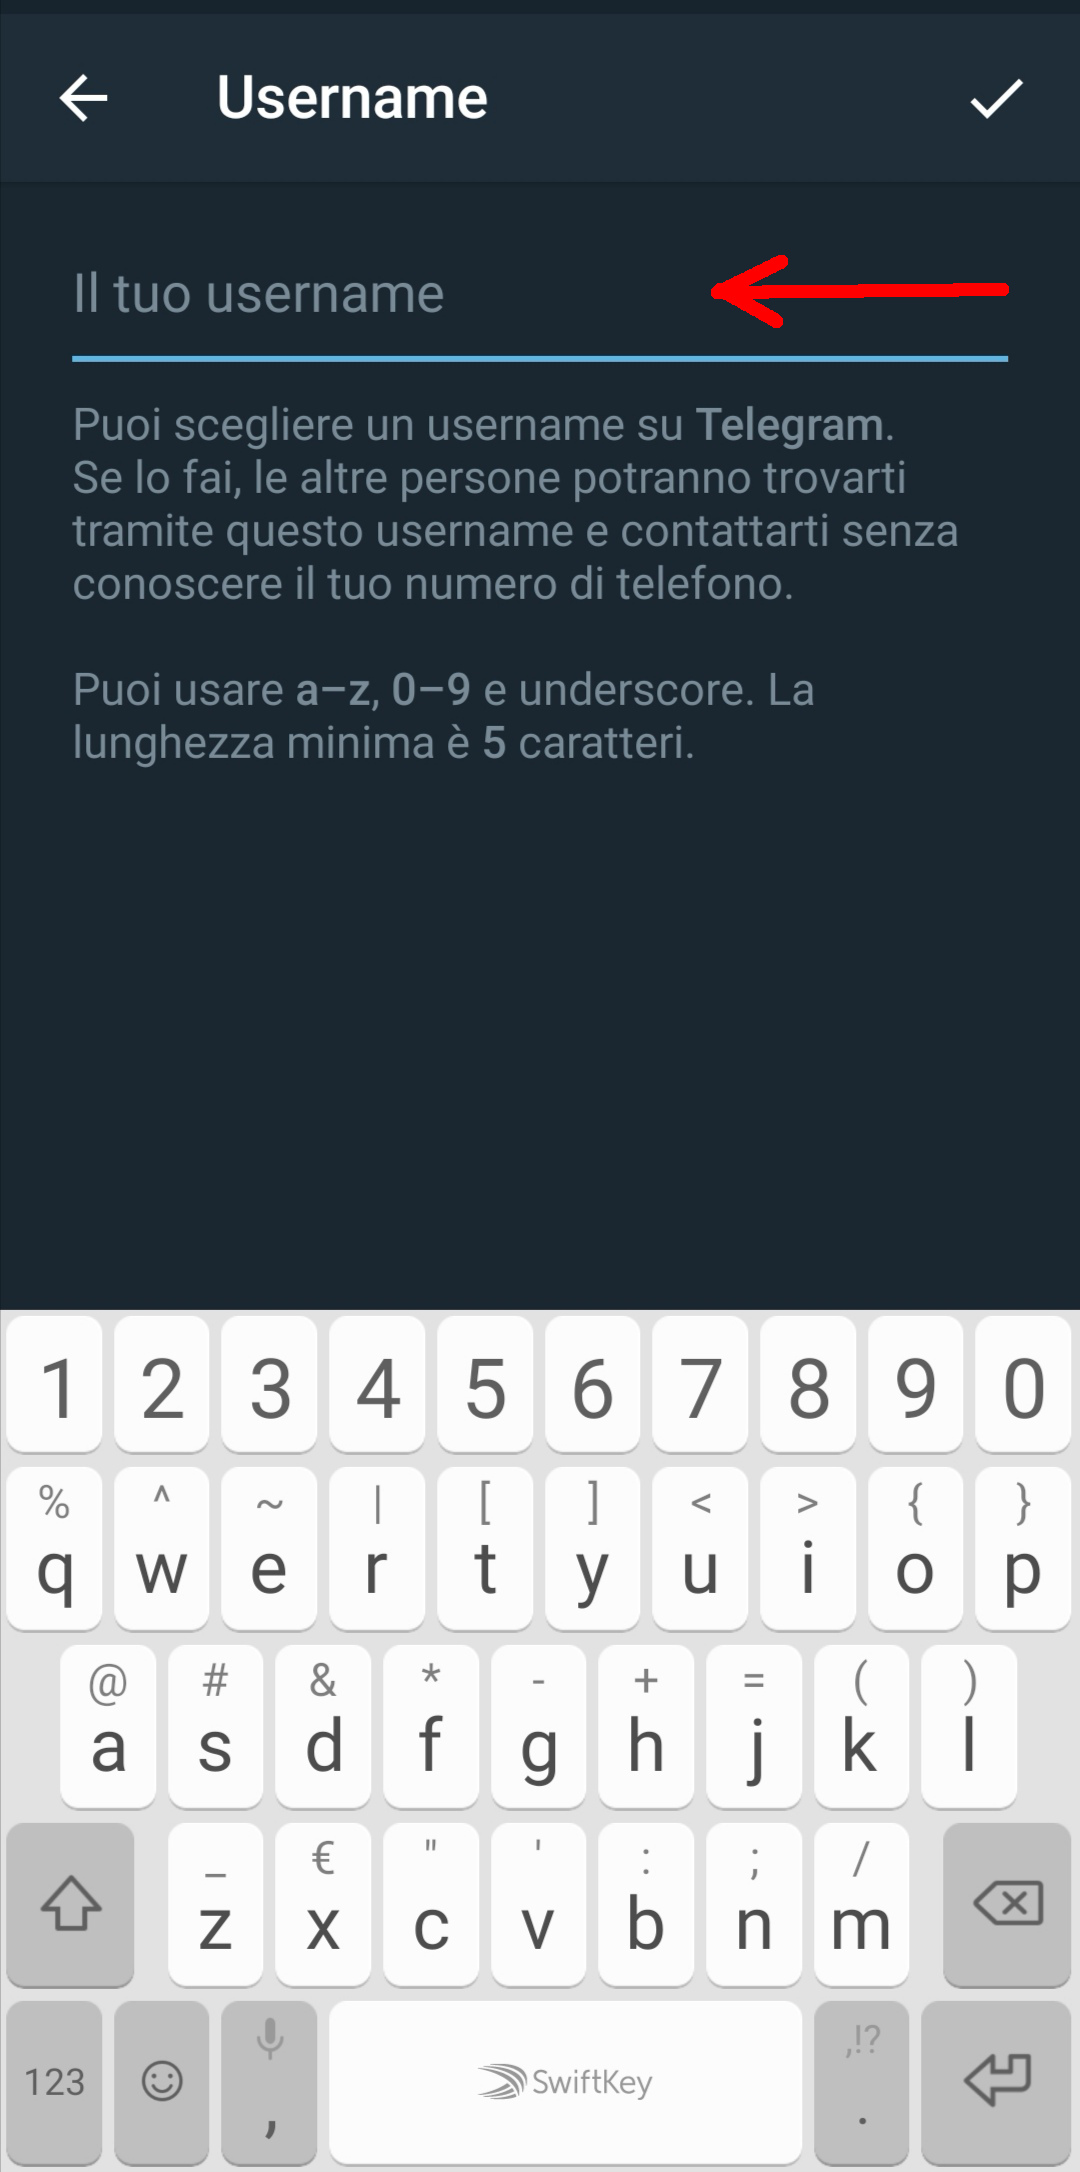
\includegraphics[scale=0.100]{res/images/telegram3.jpg}
		\caption{Come salvare lo username inserito}
		\label{Screenshot3}
	\end{figure}

\subsection{Abilitazione notifiche alert e TFA}
Per visualizzare il tutorial recati al seguente link: 
\url{}

\subsection{Alerts e impostazioni di notifica}
Per visualizzare il tutorial recati al seguente link: 
\url{}

\subsection{Gestione pagine view}
Per visualizzare il tutorial recati al seguente link: 
\url{}

\subsection{Gestione dispositivi e sensori}
Per visualizzare il tutorial recati al seguente link: 
\url{}

